%% bare_conf.tex
%% This is a skeleton file demonstrating the use of IEEEtran.cls
%% (requires IEEEtran.cls version 1.7 or later) with an IEEE conference paper.

%\documentclass[conference]{IEEEtran}
\documentclass[conference,10pt,draftclsnofoot,onecolumn]{IEEEtran}
\newcommand{\BEAS}{\begin{eqnarray*}}
\newcommand{\EEAS}{\end{eqnarray*}}
\newcommand{\BEQ}{\begin{equation}}
\newcommand{\EEQ}{\end{equation}}
\newcommand{\BIT}{\begin{itemize}}
\newcommand{\EIT}{\end{itemize}}

\newcommand{\eg}{{\it e.g.\ }}
\newcommand{\ie}{{\it i.e.\ }}

\newcommand{\ones}{\mathbf 1}
\newcommand{\zeros}{\mathbf 0}
\newcommand{\reals}{{\mbox{\bf R}}}
\newcommand{\integers}{{\mbox{\bf Z}}}
\newcommand{\symm}{{\mbox{\bf S}}}  % symmetric matrices

\newcommand{\nullspace}{{\mathcal N}}
\newcommand{\range}{{\mathcal R}}
\newcommand{\Rank}{\mathop{\bf Rank}}
\newcommand{\Tr}{\mathop{\bf Tr}}

\newcommand{\sign}[1]{\mathop{\textrm{sgn}}(#1)}
\newcommand{\lambdamax}{{\lambda_{\rm max}}}
\newcommand{\lambdamin}{\lambda_{\rm min}}

\newcommand{\EE}{\mathop{\textrm{E}}}
\newcommand{\Cov}{\mathop{\textrm{Cov}}}
\newcommand{\Prob}{\mathop{\bf Prob}}
\newcommand{\Co}{{\mathop {\bf Co}}} % convex hull
\newcommand{\dist}{\mathop{\bf dist{}}}
\newcommand{\argmin}{\mathop{\rm argmin}}
\newcommand{\argmax}{\mathop{\rm argmax}}
\newcommand{\epi}{\mathop{\bf epi}} % epigraph
\newcommand{\Vol}{\mathop{\bf vol}}
\newcommand{\dom}{\mathop{\bf dom}} % domain
\newcommand{\intr}{\mathop{\bf int}}


\newcommand{\nrm}[1]{\left\lVert#1\right\rVert}
\newcommand{\nrmo}[1]{\left\lVert#1\right\rVert_1}
\newcommand{\nrmt}[1]{\left\lVert#1\right\rVert_2}
\newcommand{\nrmnn}[1]{\left\lVert#1\right\rVert_{*}}
\newcommand{\nrmf}[1]{\left\lVert#1\right\rVert_F}

\newcommand{\myexp}[1]{\mathop{\rm exp}\left\{#1\right\}}
\newcommand{\mylog}[1]{\mathop{\rm log}\left\{#1\right\}}
\newcommand{\questions}{\begin{frame}Questions?\end{frame}}
\newcommand{\LL}{\textrm{LL}}
\newcommand{\KL}{\textrm{KL}}
\newcommand{\HH}{\textrm{H}}
\newcommand{\GG}{\textrm{G}}

\newcommand{\Bound}{\textrm{B}}
\newcommand{\bb}{\mathbf{b}}
\newcommand{\aaa}{\mathbf{a}}
\newcommand{\BB}{\mathbf{B}}
\newcommand{\AAA}{\mathbf{A}}
\newcommand{\CC}{\mathbf{C}}
\newcommand{\cc}{\mathbf{c}}
\newcommand{\mm}{\mathbf{m}}
\newcommand{\MM}{\mathbf{M}}
\newcommand{\nn}{\mathrm{\bf neighbors}}
\newcommand{\pa}[1]{{\textrm{\bf pa}}\left(#1\right)}
\newcommand{\pre}[2]{\mathop{\textrm{\bf pnp}}_{#1}\left(#2\right)}
\newcommand{\logsum}{\textrm{logsum}}

\newcommand{\tth}{{\textrm{th}}}
\newcommand{\xx}{\mathbf{x}}
\newcommand{\mmu}{\mathbf{\mu}}
\newcommand{\yy}{\mathbf{y}}
\newcommand{\zz}{\mathbf{z}}
\newcommand{\dd}{\mathbf{d}}
\newcommand{\new}{\textrm{new}}
\newcommand{\old}{\textrm{old}}
\newcommand{\fpr}{\textrm{FPR}}
\newcommand{\tpr}{\textrm{TPR}}
\newcommand{\auc}{\textrm{AUC}}
\newcommand{\yyi}{\yy_i}
\newcommand{\xxi}{\xx_i}
\newcommand{\vvec}[2]{\left[ \begin{array}{c} \mathbf{#1}\\ \mathbf{#2} \end{array}\right]}
\newcommand{\mmat}[4]{\left[ \begin{array}{cc} \mathbf{#1}&\mathbf{#2}\\ \mathbf{#3}&\mathbf{#4} \end{array}\right]}
\newcommand{\xyvec}{\left[ \begin{array}{c} \xx\\\yy \end{array} \right]}
\newcommand{\xyvecc}{\left[ \begin{array}{c} x^1\\y^1 \end{array} \right]}
\newcommand{\eye}{   \left[ \begin{array}{cc} 1 & 0 \\ 0 & 1 \end{array}\right]}
\newcommand{\bket}[2]{\left\langle#1,#2\right\rangle}
\newcommand{\bbket}[2]{\left\llangle#1,#2\right\rrangle}
\newcommand{\redq}{\textcolor{red}{q}}
\newcommand{\blup}{\textcolor{blue}{p}}
\newcommand{\BIEA}{\begin{IEEEeqnarray*}}
\newcommand{\EIEA}{\end{IEEEeqnarray*}}
\newcommand{\BIEAN}{\begin{IEEEeqnarray}}
\newcommand{\EIEAN}{\end{IEEEeqnarray}}
\newcommand{\pmin}{\mathop{\textrm{minimize}}}
\newcommand{\psubjto}{\textrm{subject to}}
\newcommand{\WW}{\mathbf{W}}
\newcommand{\ww}{\mathbf{w}}
\newcommand{\YY}{\mathbf{Y}}
\newcommand{\XX}{\mathbf{X}}
\newcommand{\UU}{\mathbf{U}}
\newcommand{\uu}{\mathbf{u}}
\newcommand{\VV}{\mathbf{V}}
\newcommand{\vv}{\mathbf{v}}
\newcommand{\PP}{\mathbf{P}}
\newcommand{\pp}{\mathbf{p}}
\newcommand{\rr}{\mathbf{r}}
\newcommand{\RR}{\mathbf{R}}
\newcommand{\ee}{\mathbf{e}}
\newcommand{\II}{\mathbf{I}}
\newcommand{\DD}{\mathbf{D}}

\newcommand{\aalpha}{{\boldsymbol\alpha}}
\newcommand{\llambda}{{\boldsymbol\lambda}}
\newcommand{\ddelta}{{\boldsymbol\delta}}
\newcommand{\otherwise}{\textrm{otherwise}}
\newcommand{\answer}{\fbox{\tt answer} }
\newcommand{\abs}[1]{\left| #1 \right|}

\newcounter{problemCtr}
\newcommand{\newproblem}[1]{\hrule\paragraph{Problem \theproblemCtr (#1)}\stepcounter{problemCtr}}


\newcounter{HW}

\usepackage{amsthm}
\usepackage{graphicx}
\usepackage{natbib}
\usepackage{algorithm}
\usepackage{algorithmic}
\usepackage{amsmath}
\usepackage{hyperref}
\usepackage{tikz}


\newtheorem{remark}{Remark}
\newtheorem{lemma}{Lemma}
\newtheorem{definition}{Definition}
\newtheorem{proposition}{Proposition}
\newtheorem{assumption}{Assumption}
\newtheorem{corollary}{Corollary}
\newtheorem{theorem}{Theorem}



% *** MISC UTILITY PACKAGES ***
% *** CITATION PACKAGES ***
\usepackage{cite}
% cite.sty was written by Donald Arseneau
% V1.6 and later of IEEEtran pre-defines the format of the cite.sty package
% \cite{} output to follow that of IEEE. Loading the cite package will
% result in citation numbers being automatically sorted and properly
% "compressed/ranged". e.g., [1], [9], [2], [7], [5], [6] without using
% cite.sty will become [1], [2], [5]--[7], [9] using cite.sty. cite.sty's
% \cite will automatically add leading space, if needed. Use cite.sty's
% noadjust option (cite.sty V3.8 and later) if you want to turn this off.
% cite.sty is already installed on most LaTeX systems. Be sure and use
% version 4.0 (2003-05-27) and later if using hyperref.sty. cite.sty does
% not currently provide for hyperlinked citations.
% The latest version can be obtained at:
% http://www.ctan.org/tex-archive/macros/latex/contrib/cite/
% The documentation is contained in the cite.sty file itself.

% *** GRAPHICS RELATED PACKAGES ***
%
\ifCLASSINFOpdf
   \usepackage[pdftex]{graphicx}
  % declare the path(s) where your graphic files are
  % \graphicspath{{../pdf/}{../jpeg/}}
  % and their extensions so you won't have to specify these with
  % every instance of \includegraphics
  % \DeclareGraphicsExtensions{.pdf,.jpeg,.png}
\else
  % or other class option (dvipsone, dvipdf, if not using dvips). graphicx
  % will default to the driver specified in the system graphics.cfg if no
  % driver is specified.
   \usepackage[dvips]{graphicx}
  % declare the path(s) where your graphic files are
  % \graphicspath{{../eps/}}
  % and their extensions so you won't have to specify these with
  % every instance of \includegraphics
  % \DeclareGraphicsExtensions{.eps}
\fi
% You can find documentation about the pdfTeX application at:
% http://www.tug.org/applications/pdftex

% *** MATH PACKAGES ***
%
\usepackage[cmex10]{amsmath}

% A popular package from the American Mathematical Society that provides
% many useful and powerful commands for dealing with mathematics. If using
% it, be sure to load this package with the cmex10 option to ensure that
% only type 1 fonts will utilized at all point sizes. Without this option,
% it is possible that some math symbols, particularly those within
% footnotes, will be rendered in bitmap form which will result in a
% document that can not be IEEE Xplore compliant!
%
% Also, note that the amsmath package sets \interdisplaylinepenalty to 10000
% thus preventing page breaks from occurring within multiline equations. Use:
%\interdisplaylinepenalty=2500
% after loading amsmath to restore such page breaks as IEEEtran.cls normally
% does. amsmath.sty is already installed on most LaTeX systems. The latest
% version and documentation can be obtained at:
% http://www.ctan.org/tex-archive/macros/latex/required/amslatex/math/

% *** SPECIALIZED LIST PACKAGES ***
%
\usepackage{algorithmicx, algorithm, algpseudocode}
\usepackage{algpseudocode}
% algorithmic.sty was written by Peter Williams and Rogerio Brito.
% This package provides an algorithmic environment fo describing algorithms.
% You can use the algorithmic environment in-text or within a figure
% environment to provide for a floating algorithm. Do NOT use the algorithm
% floating environment provided by algorithm.sty (by the same authors) or
% algorithm2e.sty (by Christophe Fiorio) as IEEE does not use dedicated
% algorithm float types and packages that provide these will not provide
% correct IEEE style captions. The latest version and documentation of
% algorithmic.sty can be obtained at:
% http://www.ctan.org/tex-archive/macros/latex/contrib/algorithms/
% There is also a support site at:
% http://algorithms.berlios.de/index.html
% Also of interest may be the (relatively newer and more customizable)
% algorithmicx.sty package by Szasz Janos:
% http://www.ctan.org/tex-archive/macros/latex/contrib/algorithmicx/

% *** ALIGNMENT PACKAGES ***
%
\usepackage{array}
% Frank Mittelbach's and David Carlisle's array.sty patches and improves
% the standard LaTeX2e array and tabular environments to provide better
% appearance and additional user controls. As the default LaTeX2e table
% generation code is lacking to the point of almost being broken with
% respect to the quality of the end results, all users are strongly
% advised to use an enhanced (at the very least that provided by array.sty)
% set of table tools. array.sty is already installed on most systems. The
% latest version and documentation can be obtained at:
% http://www.ctan.org/tex-archive/macros/latex/required/tools/


\usepackage{mdwmath}
\usepackage{mdwtab}
% Also highly recommended is Mark Wooding's extremely powerful MDW tools,
% especially mdwmath.sty and mdwtab.sty which are used to format equations
% and tables, respectively. The MDWtools set is already installed on most
% LaTeX systems. The lastest version and documentation is available at:
% http://www.ctan.org/tex-archive/macros/latex/contrib/mdwtools/


% IEEEtran contains the IEEEeqnarray family of commands that can be used to
% generate multiline equations as well as matrices, tables, etc., of high
% quality.


%\usepackage{eqparbox}
% Also of notable interest is Scott Pakin's eqparbox package for creating
% (automatically sized) equal width boxes - aka "natural width parboxes".
% Available at:
% http://www.ctan.org/tex-archive/macros/latex/contrib/eqparbox/


% *** SUBFIGURE PACKAGES ***
\usepackage[tight,footnotesize]{subfigure}
% subfigure.sty was written by Steven Douglas Cochran. This package makes it
% easy to put subfigures in your figures. e.g., "Figure 1a and 1b". For IEEE
% work, it is a good idea to load it with the tight package option to reduce
% the amount of white space around the subfigures. subfigure.sty is already
% installed on most LaTeX systems. The latest version and documentation can
% be obtained at:
% http://www.ctan.org/tex-archive/obsolete/macros/latex/contrib/subfigure/
% subfigure.sty has been superceeded by subfig.sty.

%\usepackage[font=footnotesize]{subfig}
% subfig.sty, also written by Steven Douglas Cochran, is the modern
% replacement for subfigure.sty. However, subfig.sty requires and
% automatically loads Axel Sommerfeldt's caption.sty which will override
% IEEEtran.cls handling of captions and this will result in nonIEEE style
% figure/table captions. To prevent this problem, be sure and preload
% caption.sty with its "caption=false" package option. This is will preserve
% IEEEtran.cls handing of captions. Version 1.3 (2005/06/28) and later 
% (recommended due to many improvements over 1.2) of subfig.sty supports
% the caption=false option directly:
%\usepackage[caption=false,font=footnotesize]{subfig}
%
% The latest version and documentation can be obtained at:
% http://www.ctan.org/tex-archive/macros/latex/contrib/subfig/
% The latest version and documentation of caption.sty can be obtained at:
% http://www.ctan.org/tex-archive/macros/latex/contrib/caption/


% *** FLOAT PACKAGES ***
%
\usepackage{fixltx2e}
% fixltx2e, the successor to the earlier fix2col.sty, was written by
% Frank Mittelbach and David Carlisle. This package corrects a few problems
% in the LaTeX2e kernel, the most notable of which is that in current
% LaTeX2e releases, the ordering of single and double column floats is not
% guaranteed to be preserved. Thus, an unpatched LaTeX2e can allow a
% single column figure to be placed prior to an earlier double column
% figure. The latest version and documentation can be found at:
% http://www.ctan.org/tex-archive/macros/latex/base/

\usepackage{stfloats}
% stfloats.sty was written by Sigitas Tolusis. This package gives LaTeX2e
% the ability to do double column floats at the bottom of the page as well
% as the top. (e.g., "\begin{figure*}[!b]" is not normally possible in
% LaTeX2e). It also provides a command:
%\fnbelowfloat
% to enable the placement of footnotes below bottom floats (the standard
% LaTeX2e kernel puts them above bottom floats). This is an invasive package
% which rewrites many portions of the LaTeX2e float routines. It may not work
% with other packages that modify the LaTeX2e float routines. The latest
% version and documentation can be obtained at:
% http://www.ctan.org/tex-archive/macros/latex/contrib/sttools/
% Documentation is contained in the stfloats.sty comments as well as in the
% presfull.pdf file. Do not use the stfloats baselinefloat ability as IEEE
% does not allow \baselineskip to stretch. Authors submitting work to the
% IEEE should note that IEEE rarely uses double column equations and
% that authors should try to avoid such use. Do not be tempted to use the
% cuted.sty or midfloat.sty packages (also by Sigitas Tolusis) as IEEE does
% not format its papers in such ways.

% *** PDF, URL AND HYPERLINK PACKAGES ***
%
\usepackage{url}
% url.sty was written by Donald Arseneau. It provides better support for
% handling and breaking URLs. url.sty is already installed on most LaTeX
% systems. The latest version can be obtained at:
% http://www.ctan.org/tex-archive/macros/latex/contrib/misc/
% Read the url.sty source comments for usage information. Basically,
% \url{my_url_here}.

% *** Do not adjust lengths that control margins, column widths, etc. ***
% *** Do not use packages that alter fonts (such as pslatex).         ***
% There should be no need to do such things with IEEEtran.cls V1.6 and later.
% (Unless specifically asked to do so by the journal or conference you plan
% to submit to, of course. )

% custom packages
\usepackage{verbatim}
\usepackage{multirow}
\usepackage{hhline}

% start document
\begin{document}
%
% paper title
% can use linebreaks \\ within to get better formatting as desired
\title{Prediction of MHC Class II binding peptides incorporating bayesian transfer hierarchies}

% author names and affiliations
% use a multiple column layout for up to three different
% affiliations
\author{\IEEEauthorblockN{Ravikiran Janardhana}
\IEEEauthorblockA{Department of Computer Science\\
University of North Carolina at Chapel Hill\\
Email: ravikirn@cs.unc.edu}
}

% make the title area
\maketitle

\begin{abstract}
T-cells are key players in regulating a specific immune response. Activation of
cytotoxic T-cells requires recognition of specific peptides bound to Major Histocompatibility
Complex (MHC) class II molecules. MHC-peptide complexes are potential tools for diagnosis and
treatment of pathogens and cancer, as well as for the development of peptide vaccines. Only one
in 100 to 200 potential binders actually binds to a certain MHC molecule, therefore a good
prediction method for MHC class II binding peptides can reduce the number of candidate binders
that need to be synthesized and tested for successful design of peptide and protein based vaccines.
\end{abstract}

%\begin{IEEEkeywords}
%MHC class II, peptide prediction, bayesian transfer hierarchy
%\end{IEEEkeywords}

\section{Introduction}
The activation of CD4+ helper T cells is essential for the development of adaptive immunity against pathogens \cite{jenkins01}. A
critical step in CD4+ T cell activation is the recognition of epitopes presented by MHC class II molecules \cite{rudolph06}. MHC class II molecules
are heterodimers expressed on the surface of professional antigen presenting cells that bind peptide fragments derived from protein
antigens. X-ray crystallographic studies demonstrated that the MHC class II epitope binding site consists of a groove and several
pockets provided by a $\beta$-sheet and two $\alpha$-helices. Unlike class I, the class II binding groove is open at both ends. As a result,
peptides binding to class II molecules tend to be of variable length, but typically between 13 and 25 residues.

A hallmark of the MHC class II binding peptide groove is that there are four major pockets. These pockets accommodate side chains of
residues 1, 4, 6, and 9 of a 9-mer core region of the binding peptide. This core region interaction largely determines binding affinity
and specificity \cite{jones06}. In addition, peptide residues immediately flanking the core region have been indicated to make contact with the
MHC molecule outside of the binding groove, and to contribute to MHC-peptide interaction.  MHC class II molecules are highly polymorphic, and this
polymorphism largely corresponds with differences along the peptide binding groove. However, the binding motifs derived for
MHC class II molecules are highly degenerate, and many promiscuous peptides have been identified that can bind multiple
MHC class II molecules. Promiscuous peptides are a prime target for vaccine and immunotherapy and computational tools
have been developed to facilitate systematic scanning for promiscuous peptides.

Computational prediction of MHC class II epitopes is of important theoretical and practical value, as experimental dentification
is costly and time consuming. Many computational methods exist to predict peptide MHC binding. Experimentally determined affinities
data have formed the basis of many peptide-MHC binding prediction methods and has enabled classification of binding and
nonbinding peptides. Highly sophisticated computer science algorithms such as artificial neural networks \cite{gulukota00},
HMMs \cite{noguchi02}, support vector machines (SVMs) \cite{wan06} and methods derived from computational chemistry,
such as QSAR analysis \cite{doytchinova05} and structure-based approaches \cite{davies06} have been previous deployed to solve this problem.

Dimitrov et al. \cite{dimitrov10} and Wang et al. \cite{wang08} have published detailed assessment of MHC Class II peptide binding
predictors. In the above mentioned assessment, it was clear that each predictor for a specific genetic loci (including its alleles)
worked independently i.e., no knowledge sharing occured between predictors although they might be predicting alleles of the same genetic loci.
In this project, I propose that the prediction of MHC Class II alleles of the same genetic loci (HLA-DR*, HLA-DQ* and HLA-DP*) are dependent
on each other since these alleles are nothing but an alternative form of the same gene. I tie pairs of MHC Class II alleles together and jointly
learn the prediction/classifier parameters. This approach allows for transfer learning via high dimensional bayesian transfer hierarchies \cite{elidan08}.
My results are then compared to the state of the art support vector machine methods \cite{wan06}, GLMNET \cite{friedman09}
and I show that our joint classifier either matches or outperforms the SVM and GLMNET methods consistently.

%In the remaining sections, I describe the dataset in \ref{subsec:dataset}, features in \ref{subsec:features},
%optimization setup in \ref{subsec:optimization} and the overall algorithm in \ref{subsec:algorithm}.
%In Section \ref{sec:results}, I discuss the experimental results and conclusion in Section \ref{sec:conclusion}.

\section{Method}
\label{sec:method}
In the proposed method, pairs of MHC Class II alleles of the same genetic locus are paired together and I train a joint classifier on both to predict the
binding and non-binding peptides. The following subsections describes the optimization setup and the algorithm of my method.

\subsection{Optimization Setup}
\label{subsec:optimization}
The optimization problem for logistic regression with a fused lasso penalty for a single predictor is given as
\begin{align}
\label{eqn1}
\mathop{\textrm{minimize}}_{\ww} & \sum_i \mylog{1 + \myexp{-y_i(\xx_i\ww)}} + \lambda\nrmo{\ww} + \mu\nrmo{\DD\ww}.
\end{align}

%\BEAS
%\mathop{\textrm{minimize}}_{\ww} && \sum_i \mylog{1 + \myexp{-y_i(\xx_i\ww)}} + \lambda\nrmo{\ww} + \mu\nrmo{\DD\ww}.
%\EEAS

where,
\[
%\ww = \begin{bmatrix} w_{1} & w_{2} & \cdots & w_{n} \end{bmatrix}^\top 
%\textrm{and }
\xx, \yy, \ww \in \RR^n, 
\textrm{ and }
\DD = \begin{bmatrix}   1 & 0 & \cdots & 0 & -1 & 0 & \cdots & 0\\
                        0 & 1 & \cdots & 0 & 0 & -1 & \cdots & 0\\
                        \vdots & \vdots & \ddots & \vdots & \vdots & \vdots & \ddots & \vdots\\
                        0 & 0 & \cdots & 1 & 0 & 0 & \cdots & -1 
      \end{bmatrix}
\]

Since, we want to build a joint classifier for a pair of predictors and want to impose a constraint on the weights of both of their features,
the optimization problem in \eqref{eqn1} is modified as below:-

\begin{align}
\label{eqn2}
\mathop{\textrm{minimize}}_{\ww^{1}, \ww^{2}} & \sum_i \mylog{1 + \myexp{-y^{1}_i(\xx^{1}_i\ww^{1})}} + \sum_i \mylog{1 + \myexp{-y^{2}_i(\xx^{2}_i\ww^{2})}} \\
                                              & + \lambda_{1}\nrmo{\ww^{1}} + \lambda_{2}\nrmo{\ww^{2}} + \mu\nrmo{\DD\ww} \notag.
\end{align}

where,
\[
\ww = \begin{bmatrix} \ww^{1} & \ww^{2}\end{bmatrix}^\top
\]


Equation \eqref{eqn2} can be further simplified by packing variables $\yy^1$ and $\yy^2$ into $\yy$, $\xx^1$ and $\xx^2$ into $\xx$ and suitably modifying $\DD$ as below:-
\begin{align}
\label{eqn3}
\mathop{\textrm{minimize}}_{\ww} & \sum_i \mylog{1 + \myexp{-y_i(\xx_i\ww)}} + \mu\nrmo{\DD\ww}.
\end{align}

where,
\[
    \DD = \begin{bmatrix}   \mu & 0 & \cdots & 0 & -\mu & 0 & \cdots & 0\\
    0 & \mu & \cdots & 0 & 0 & -\mu & \cdots & 0\\
    \vdots & \vdots & \ddots & \vdots & \vdots & \vdots & \ddots & \vdots\\
    0 & 0 & \cdots & \mu & 0 & 0 & \cdots & -\mu \\
    \lambda_1 & 0 & \cdots & 0 & \lambda_2 & 0 & \cdots & 0\\
    0 & \lambda_1 & \cdots & 0 & 0 & \lambda_2 & \cdots & 0\\
    \vdots & \vdots & \ddots & \vdots & \vdots & \vdots & \ddots & \vdots\\
    0 & 0 & \cdots & \lambda_1 & 0 & 0 & \cdots & \lambda_2
    \end{bmatrix}\\
    \textrm{ ,  }\\
    \yy = \begin{bmatrix} \yy^{1} \\ \yy^{2}\end{bmatrix}\\
    \textrm{ ,  }\\
    \xx = \begin{bmatrix} \xx^{1} & 0 \\ 0 & \xx^{2}\end{bmatrix}\\
    \textrm{ and  }\\
    \ww = \begin{bmatrix} \ww^{1} \\ \ww^{2}\end{bmatrix}
\]

Writing out the augmented lagrangian for \eqref{eqn3},
\begin{align}
\label{eqn4}
AL(\ww, \zz^0, \zz^1, \uu^0, \uu^1) = & \sum_i \log\{1+\exp\{-y_{i}z_{i}^{0}\}\} + \mu\nrmo{\zz^1} + \notag \\
& \sum_{i} u_{i}^{0} (z_{i}^{0} - \xx_{i}\ww) + \uu^{1} (\zz^{1} - \DD\ww) + \\
& \sum_{i} \frac{\rho}{2} \nrmt{z_{i}^{0} - \xx_{i}\ww}^{2} + \frac{\rho}{2} \nrmt{\zz^{1} - \DD\ww}^{2} \notag
\end{align}

We can solve the above augmented lagrangian using alternating direction method of multipliers (ADMM) \cite{jojic12}. The ADMM algorithm
iterates following updates,
\begin{align}
    \label{eqn5}
    \ww^k = & \mathop{\textrm{ argmin}}_\ww AL(\ww, \zz^{0, k-1}, \zz^{1, k-1}, \uu^{0, k-1}, \uu^{1, k-1}) \notag\\
    \zz^{0, k} = & \mathop{\textrm{ argmin}}_\ww AL(\ww^k, \zz^{0}, \zz^{1, k-1}, \uu^{0, k-1}, \uu^{1, k-1})\notag\\
    \zz^{1, k} = & \mathop{\textrm{ argmin}}_\ww AL(\ww^k, \zz^{0, k}, \zz^{1}, \uu^{0, k-1}, \uu^{1, k-1}) \\
    \uu^{0, k} = & \uu^{0, k-1} + \rho (\zz^{0, k} - \ww^k) \notag\\
    \uu^{1, k} = & \uu^{1, k-1} + \rho (\zz^{0, k} - \DD\ww^k)\notag
\end{align}
where $k - 1$ and $k$ denote previous and current iteration respectively.

Now, we derive the updates for $\ww^k, \zz^{0, k}, \zz^{1, k}$

\subsubsection{Deriving update for \textbf{w}$^k$}
\label{subsubsec:wupdate}
Eliminating terms that are constants with respect to $\ww$ and completing the squares we obtain,
\begin{align}
\label{eqn6}
\ww^k =& \argmin_\ww \frac{\rho}{2} \nrmt{\begin{bmatrix} \xx \\ \DD \end{bmatrix}\ww - \begin{bmatrix} \zz^{0,k-1} + \frac{1}{\rho} \uu^{0, k-1} \\ \zz^{1,k-1} + \frac{1}{\rho} \uu^{1, k-1} \end{bmatrix} }^{2} 
\end{align}

Thus, an update for $\ww$ requires solving the above system of linear equations.

\subsubsection{Deriving update for \textbf{z}$^{0, k}$}
\label{subsubsec:z0update}

\begin{align}
\label{eqn7}
z_i^{0,k} = & \argmin_{z_i^0}   \log{\{1+exp\{-y_{i}z_{i}^{0}\}\}} + \frac{\rho}{2}\nrmt{z_{i}^{0} - (\xx_{i}\ww^{k}-\frac{1}{\rho}u_{i}^{0,k-1})}^{2} 
\end{align}

Since $\zz^{0}$ is scalar, the objective is univariate. We can solve the above unconstrained optimization using Newton algorithm
with backtracking and the weak Wolfe condition for backtracking termination \cite{burke12}.

\subsubsection{Deriving update for \textbf{z}$^{1, k}$}
\label{subsubsec:z1update}

\begin{align}
\label{eqn8}
z_i^{1,k} = & \argmin_{z_i^1} \frac{\mu}{\rho} \nrmo{z_{i}^{1}} + \frac{1}{2} \nrmt{z_{i}^{1} - \DD\ww^{k} + \frac{1}{\rho}u_{i}^{1,k-1}}^{2} 
\end{align}

The above optimization can be solved in a closed form 
\begin{align}
\label{eqn9}
z_i^{1,k} = & S(\DD\ww^{k} - \frac{1}{\rho}u_{i}^{1, k-1}, \frac{\mu}{\rho}) 
\end{align}

where \textbf{S} is the Shrink Threshold operator defined as below,
\begin{align}
\label{eqn10}
S(x, \lambda) = & sign(x) \textrm{  } max (|x| - \lambda, 0)
\end{align}

The updates for the dual variables $\uu^{0,k}$ and $\uu^{1,k}$ are already listed in equation \eqref{eqn5}.

\subsection{Algorithm}
Putting all of the updates listed in Section \ref{subsec:optimization} together, we can compute '$\ww$' using the steps listed in algorithm \ref{algo:fusedADMM}. In this
algorithm, due to the vast feature space, we will iterate only for a maximum of 100 iterations instead until convergence.

\begin{algorithm}                      
\caption{Fused ADMM Optimization Solver}
\label{algo:fusedADMM}
\begin{algorithmic}
\Statex
\Statex {\textbf{INPUT:} $\yy$, $\XX$, $\DD$, $\lambda_1$ (lambda1), $\lambda_2$ (lambda2), $\mu$ (mu)} 
\State {rho $\gets$ 1}
\State {N $\gets$ length(y); p $\gets$ size(X,2)}
\State {e $\gets$ size(D,1); w $\gets$ zeros(p,1)}
\State {z0 $\gets$ zeros(N,1); u0 $\gets$ zeros(N,1);}
\State {z1 $\gets$ zeros(e,1); u1 $\gets$ zeros(e,1);}
\State {MAXIT $\gets$ 100;}
\State {n $\gets$ size(X, 2);}
\For{$it \gets 1 \to MAXIT$}
    \State {\% computeAL method computes the augmented lagrangian value listed in equation \eqref{eqn4}}
    \State {$before \gets computeAL(y,X,D,rho,w,z0,z1,u0,u1);$}
    \State {$w \gets updatew(X, D, z0, z1, u0, u1, rho);$}
    \State {$after \gets computeAL(y,X,D,rho,w,z0,z1,u0,u1);$}
    \State {$assert(after < before + 1e-6);$}
    \Statex

    \State {$before \gets after;$}
    \For{$i \gets 1 \to length(y)$}
        \State {\% updatez0i calls a function which uses newton method with weak wolfe condition}
        \State {$z0(i) \gets updatez0i(y(i), X(i,:), w, u0(i), rho);$}
    \EndFor
    \State {$after \gets computeAL(y,X,D,rho,w,z0,z1,u0,u1);$}
    \State {$assert(after < before + 1e-6);$}
    \Statex

    \State {$before \gets after;$}
    \State {$Dw \gets D*w;$}
    \For {$i \gets 1 \to size(D,1)$}
        \State {$z1(i) \gets updatez1i(Dw(i), u1(i), mu, rho);$}
    \EndFor
    \State {$after \gets computeAL(y,X,D,rho,w,z0,z1,u0,u1);$}
    \State {$assert(after < before + 1e-6);$}
    \Statex

    \State {$u0  \gets  u0 + rho * (z0 - X*w);$}
    \State {$u1  \gets  u1 + rho * (z1 - D*w);$}
\EndFor
\Statex {\bf OUTPUT:} $\ww$
\end{algorithmic}
\end{algorithm}

\section{Experimental Results}
\label{sec:expResults}
The following subsections explain the dataset, features and the results of my method.
\subsection{Dataset}
\label{subsec:dataset}
I have used the MHC Class II dataset publicly made available by Wang et al \cite{wang08} at \cite{wangData08}. For the purposes of my experiments, I have considered 15-mers of HLA-DRB1* MHC Class-II type and filtered out the rest. The detailed split of the dataset is shown in Table \ref{tab:dataset}. For each MHC Class-II type, I have used 70\% of the data for training and 30\% for testing. Within each training and testing set, 75\% of the peptides are binding and 25\% are non-binding peptides.

\begin{table}[!t]
\caption{MHC Class II dataset}
\label{tab:dataset}
\centering
\begin{tabular}{|c||c||c||c|}
\hline
MHC Class II type & Total no. of peptides & Binding Peptides & Non-binding Peptides\\
\hline
HLA-DRB1*0301 & 502 & 368 & 134\\
\hline
HLA-DRB1*0401 & 512 & 389 & 123\\
\hline
HLA-DRB1*0404 & 449 & 370 & 79\\
\hline
HLA-DRB1*0405 & 457 & 375 & 82\\
\hline
HLA-DRB1*0701 & 505 & 402 & 103\\
\hline
HLA-DRB1*0901 & 412 & 304 & 108\\
\hline
HLA-DRB1*1101 & 520 & 400 & 120\\
\hline
HLA-DRB1*1302 & 289 & 202 & 87\\
\hline
HLA-DRB1*1501 & 520 & 388 & 132\\
\hline
\end{tabular}
\end{table}

\subsection{Features}
\label{subsec:features}
I use sparse encoding \cite{qian88} for encoding the amino acid sequence. Each amino acid of the peptide sequence is mapped in a sparse orthonormal vector space by a 20-bit vector with 19 bits set to zero and one bit set to one. Therefore a peptide, which is a sequence of M consecutive amino acid letters can be represented by the concatenation of M x 20 features. In my experimental setup, I use 15-mers of HLA-DRB1* MHC Class-II type, hence each peptide can be represented by 15 x 20 = 300 feature length vector of 0s and 1s. These features alone were not sufficient to achieve a comparitive performance, hence, in addition to these I use interaction features dependent on pairs of positions. In a 15-mer, there are 210 pairs (15 x 14) of positions (x, y) where $1 \le x \le 15, 1 \le y \le 15$ and $x \ne y$. Each pair of positions can be occupied by any pair of 20 amino acids, thus, the total number of interaction features will be 84000 (15 x 14 x 20 x 20), in which one bit is set for a particular pair presence and 0 for absence. Hence, we have a total of 84300 (300 + 84000) features per peptide represented by a series of 0s and 1s.

\subsection{Classifier Parameters}
\label{subsec:params}
For all the experiments, I fixed the classifier parameters used in my method to the following values, $\lambda_1 = 0.9, \lambda_2 = 0.9, \mu = 0.9$. Due to the vast joint feature space, I was unable to run cross-validation schemes to fine tune these parameters.

\subsection{Results}
\label{subsec:results}
\begin{figure*}
    \centering
    \subfigure[]{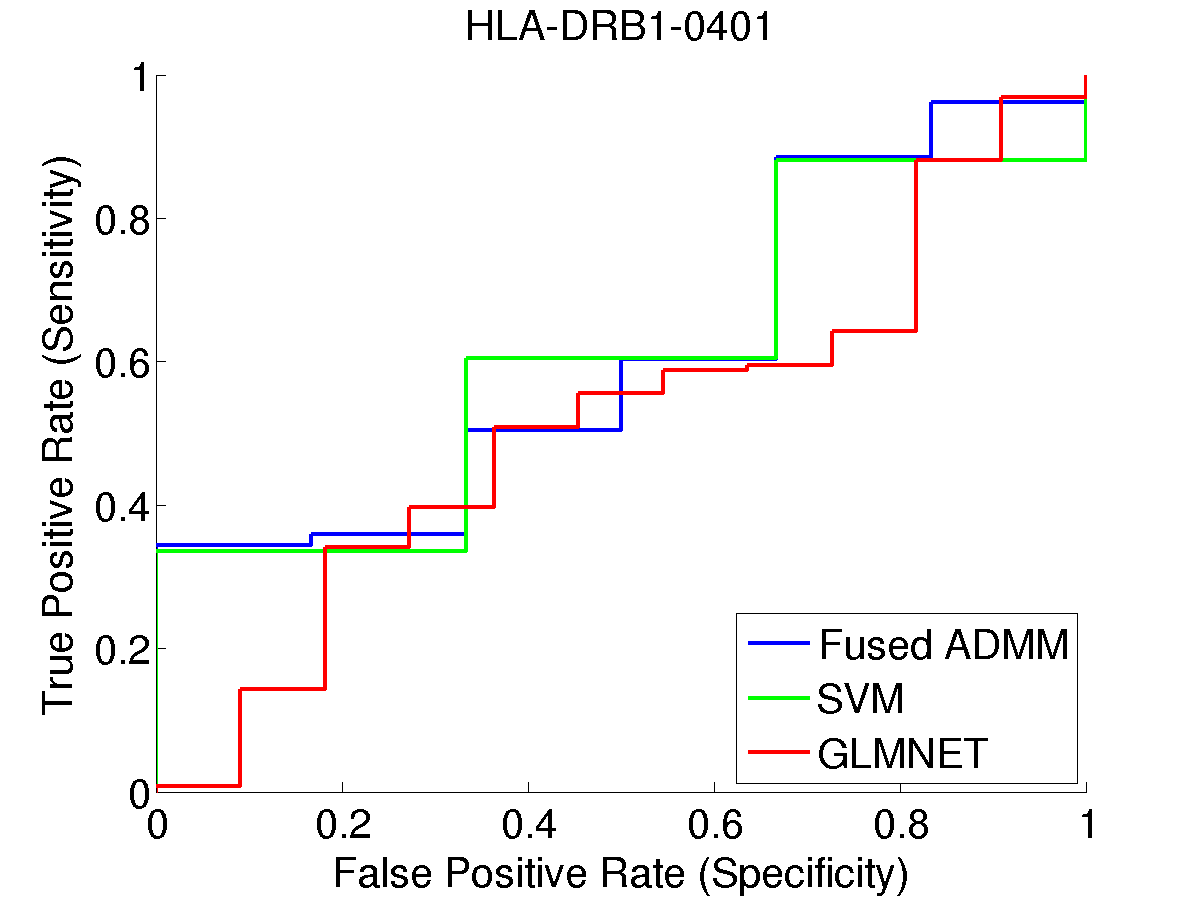
\includegraphics[width=0.49\textwidth]{images/HLA-DRB1-0401.png}\label{fig:drb1_0401}}
    \subfigure[]{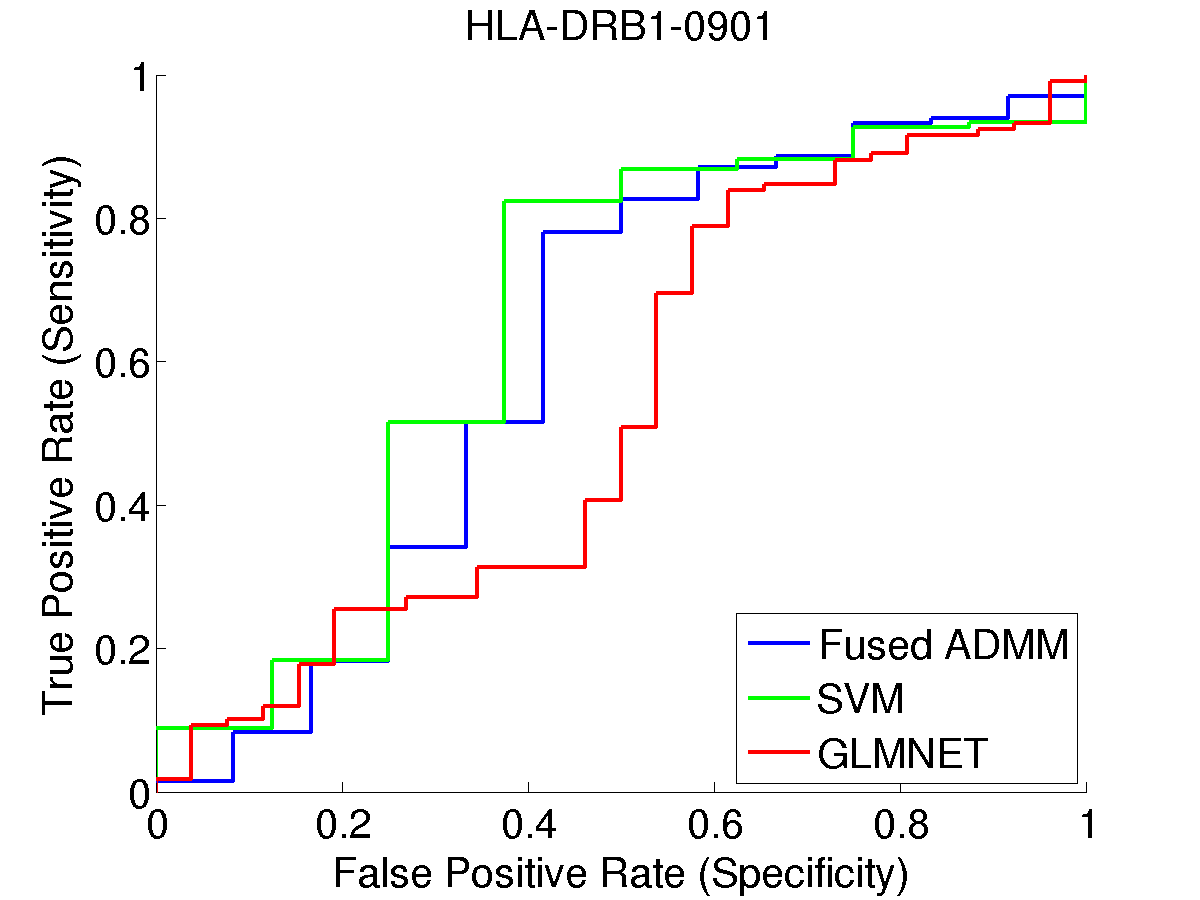
\includegraphics[width=0.49\textwidth]{images/HLA-DRB1-0901.png}\label{fig:drb1_0901}}
    \caption{Prediction results of Fused ADMM, SVM and GLMNet methods for the pair (a) HLA DRB1*0401 and (b) HLA DR1*0901 are shown in the ROC curve. The curves were generated by plotting the true positive rate (y-axis) against the false positive rate (x-axis).}
    \label{fig:roc}
\end{figure*}

\begin{table}[!t]
\caption{Results of Binding and Non-binding peptide prediction}
\label{tab:resultTable}
\centering
\begin{tabular}{|c|c|c|c|c|c|c|c|c|c|c|c|c|}
\hline
\multirow{2}{*}{MHC Class-II} & \multicolumn{3}{c|}{Precision} & \multicolumn{3}{c|}{Recall} & \multicolumn{3}{c|}{F1 Score} & \multicolumn{3}{c|}{Accuracy}\\ [2pt]
\cline{2-13}
Allele Pair & ADMM & SVM & GLM & ADMM & SVM & GLM & ADMM & SVM & GLM & ADMM & SVM & GLM \\ 
\hline

%done
\multirow{1}{*}{DRB1-0301} & \bf 0.71 & \bf 0.71 & 0.68 & \bf 0.90 & 0.89 & 0.86 & \bf 0.80 & \bf 0.80 & 0.76 & \bf 0.70 & \bf 0.70 & 0.62\\
\cline{2-13}
DRB1-0401 & \bf 0.73 & \bf 0.73 & 0.72 & 0.90 & \bf 0.91 & 0.89 & 0.80 & \bf 0.81 & 0.80 & 0.71 & \bf 0.72 & 0.68\\
%\hline
\hhline{=============}

%done
\multirow{1}{*}{DRB1-0401} & \bf 0.73 & \bf 0.73 & 0.72 & \bf 0.92 & \bf 0.92 & 0.91 & \bf 0.82 & 0.81 & 0.81 & \bf 0.72 & \bf 0.72 & 0.68\\
\cline{2-13}
DRB1-0404  & \bf 0.77 & 0.75 & 0.76 & \bf 0.92 & 0.90 & 0.90 & \bf 0.84 & 0.82 & 0.83 & \bf 0.76 & 0.74 & 0.73\\
%\hline
\hhline{=============}

%done
\multirow{1}{*}{DRB1-0401} & \bf 0.73 & \bf 0.73 & 0.72 & \bf 0.92 & \bf 0.92 & 0.91 & \bf 0.82 & 0.81 & 0.81 & \bf 0.72 & \bf 0.72 & 0.68\\
\cline{2-13}
DRB1-0405 & \bf 0.83 & \bf 0.83 & \bf 0.83 & \bf 0.92 & \bf 0.92 & 0.86 & \bf 0.87 & \bf 0.87 & 0.84 & \bf 0.83 & \bf 0.83 & 0.79\\
%\hline
\hhline{=============}

\multirow{1}{*}{DRB1-0401} & \bf 0.73 & \bf 0.73 & 0.72 & \bf 0.92 & \bf 0.92 & 0.91 & \bf 0.82 & 0.81 & 0.81 & \bf 0.72 & \bf 0.72 & 0.68\\
\cline{2-13}
DRB1-0701 & 0.78 & 0.78 & \bf 0.80 & \bf 0.92 & 0.91 & \bf 0.92 & 0.84 & 0.84 & \bf 0.85 & 0.78 & 0.78 & \bf 0.79\\
%\hline
\hhline{=============}

\multirow{1}{*}{DRB1-0401} & \bf 0.73 & \bf 0.73 & 0.72 & \bf 0.92 & \bf 0.92 & 0.91 & \bf 0.82 & 0.81 & 0.81 & \bf 0.72 & \bf 0.72 & 0.68\\
\cline{2-13}
DRB1-0901 & \bf 0.72 & 0.71 & \bf 0.72 & 0.90 & \bf 0.92 & 0.85 & \bf 0.80 & \bf 0.80 & 0.78 & \bf 0.71 & \bf 0.71 & 0.67 \\
%\hline
\hhline{=============}

\multirow{1}{*}{DRB1-0404}  & \bf 0.77 & 0.75 & 0.76 & \bf 0.92 & 0.90 & 0.90 & \bf 0.84 & 0.82 & 0.83 & \bf 0.76 & 0.74 & 0.73\\
\cline{2-13}
DRB1-0405 & \bf 0.83 & \bf 0.83 & \bf 0.83 & \bf 0.92 & \bf 0.92 & 0.86 & \bf 0.87 & \bf 0.87 & 0.84 & \bf 0.83 & \bf 0.83 & 0.79\\
%\hline
\hhline{=============}

\multirow{1}{*}{DRB1-0701} & 0.79 & 0.78 & \bf 0.80 & 0.91 & \bf 0.92 & \bf 0.92 & 0.84 & 0.84 & \bf 0.85 & 0.78 & 0.78 & \bf0.79\\
\cline{2-13}
DRB1-0901 & \bf 0.73 & 0.71 & 0.72 & 0.90 & \bf 0.92 & 0.85 & \bf 0.80 & \bf 0.80 & 0.78 & \bf 0.72 & 0.71 & 0.67\\
%\hline
\hhline{=============}

\multirow{1}{*}{DRB1-0401} & \bf 0.73 & \bf 0.73 & 0.72 & \bf 0.92 & \bf 0.92 & 0.91 & \bf 0.82 & 0.81 & 0.81 & \bf 0.72 & \bf 0.72 & 0.68\\
\cline{2-13}
DRB1-1501 & \bf 0.72 & 0.70 & 0.71 & \bf 0.92 & \bf 0.92 & 0.89 & \bf 0.80 & 0.79 & 0.79 & \bf 0.72 & 0.70 & 0.67\\
%\hline
\hhline{=============}

\multirow{1}{*}{DRB1-1101} & \bf 0.79 & 0.78 & 0.78 & \bf 0.92 & 0.91 & 0.90 & \bf 0.85 & 0.84 & 0.84 & \bf 0.80 & 0.78 & 0.77\\
\cline{2-13}
DRB1-1501 & \bf 0.72 & 0.70 & 0.71 & \bf 0.92 & \bf 0.92 & 0.89 & \bf 0.80 & 0.79 & 0.79 & \bf 0.72 & 0.70 & 0.67\\
\hline
\end{tabular}
\end{table}

I compute the standard classifier performance measures such as precision, recall, f1-score and accuracy for the 9 pairs of HLA-DRB1* MHC Class-II type alleles for my method (Fused ADMM method), SVM and GLMNET ($\alpha$ = 1.0).  These results are listed in table \ref{tab:resultTable}. The Fused ADMM method learns the weights of features on the pair of alleles jointly while SVM and GLMNET work independently on each of the pairs. From Table \ref{tab:resultTable}, it is clear that the Fused ADMM method consistently matches the performance of SVM in accuracy and outperforms it on 3 allele pairs by 1-2\% while the GLMNet method performs worse for all the pairs (lags behind by $>$ 4\%) except one w.r.t accuracy.

Figure \ref{fig:roc} shows the prediction results of Fused ADMM, SVM and GLMNET methods for the allele pair HLA DRB1*0401 and HLA DRB1*0901 in the ROC curve. The ROC curve is generated by plotting the true positive rate (sensitivity) on the y-axis against the false positive rate on the x-axis.



\section{Conclusion}
\label{sec:conclusion}
This work is concerned with the problem of classifying binding and non-binding peptide sequences w.r.t MHC Class II type alleles.
To solve this problem, I have proposed a method to jointly learn the classifier weights on an allele pair allowing transfer learning
via high dimensional bayesian transfer hierarchies. My method was evaluated and compared to SVM and GLMNet and the results showed that
it matched SVM consistently and outperformed GLMNet by a margin greater than 4\% in accuracy. For 3 allele pairs, my method performed better
than SVM slightly (1-2\%) in accuracy.

\section{Future Work}
\label{sec:futureWork}
The classifier parameters used in my method were fixed as I was not able to fine tune them due to vast joint feature space. If powerful hardware resources available,
it would be straightforward to fine tune them using cross-validations schemes and the results should improve compared to the current performance.

% use section* for acknowledgement
\section*{Acknowledgment}
I would like to thank Dr.Vladimir Jojic for his constant help during the course of this project. Without his inputs w.r.t the optimization setup, I would not have been able to solve the problem and arrive at the results.

% trigger a \newpage just before the given reference
% number - used to balance the columns on the last page
% adjust value as needed - may need to be readjusted if
% the document is modified later
%\IEEEtriggeratref{8}
% The "triggered" command can be changed if desired:
%\IEEEtriggercmd{\enlargethispage{-5in}}

% references section

% can use a bibliography generated by BibTeX as a .bbl file
% BibTeX documentation can be easily obtained at:
% http://www.ctan.org/tex-archive/biblio/bibtex/contrib/doc/
% The IEEEtran BibTeX style support page is at:
% http://www.michaelshell.org/tex/ieeetran/bibtex/
%\bibliographystyle{IEEEtran}
% argument is your BibTeX string definitions and bibliography database(s)
%\bibliography{IEEEabrv,../bib/paper}
%
% <OR> manually copy in the resultant .bbl file
% set second argument of \begin to the number of references
% (used to reserve space for the reference number labels box)
\bibliography{references}{}
\bibliographystyle{IEEEtran}

% that's all folks
\end{document}
